%This section will briefly go over what a genome-wide association study (GWAS) is, some common considerations and models. A GWAS is usually performed on a single SNP at a time, rather than all SNPs at the same time. This is due to the computational cost of analysing data sets of the sizes that are usually present in biobanks and due to there being more SNPs than individuals. There are several potential models that can be used to analyse genotypes. One method is the Cochran-Armitage test \cite{cochran1954some,armitageTest}, which tests for independence in a $ 2\times 3 $ contingency table. However, this test is not able to incorporate covariates to account for, e.g. population stratification. A regression based method is usually preferred, as it allows for covariates to be included. One downside of using regression models is the assumption that the SNP effects will be additive, which is not the case in the Cochran-Armitage test. The genetic data for regression is usually coded as $ AA = 0 $, $ Aa = 1 $, and $ aa = 2 $, where $ A $ is the major allele and $ a $ is the minor allele\cite{zeng2015statistical}. When restricting to only additive genetic effects, there is no difference between logistic or linear regression and the Cochran-Armitage test. In short, the regression methods are preferred over the Cochran-Armitage test as covariates can be included and linear regression is preferred over logistic regression, since it is more computationally efficient and there is no difference between their power\cite{sikorska2013gwas,prive2019making,balding2006tutorial}.



This section will briefly go over what a genome-wide association study (GWAS) is, some common considerations, and models used. First, we will present some commonly used model, then cover important topic for performing a GWAS, namely controlling type 1 errors, computational efficiency, and power improvement. At the end, we will also provide a non-exhaustive list of methodological advancements that excel in one or more of these topics. 


\subsection{Common GWAS models} \label{sec:GWAS:LinReg}
A GWAS is usually performed on a single SNP at a time, rather than all SNPs at the same time, meaning effect sizes are marginal instead of joint. There are several potential models that can be used to analyse genotypes, and in the early days of GWAS the Cochran-Armitage test \cite{cochran1954some,armitageTest} was used \cite{balding2006tutorial}. It has since been superseded by linear regression models, and in recent days there have been a push towards linear mixed models. These models will be presented here.


\subsubsection{Cochran-Armitage}
The Cochran-Armitage test tests for independence in a $ 2\times 3 $ contingency table. However, this test is not able to incorporate covariates to account for important covariates such as population stratification (See \cref{sec:controllingType1Errors} for details). Therefore, regression based methods become popular, as they allow for covariates to be included. If a GWAS is performed with a regression, it implicitly assumed that the genetic effect from a given SNP will be additive, which is not the case for a Cochran-Armitage test. The implicit assumption follows from how the genetic data is coded for regression as $ AA = 0 $, $ Aa = 1 $, and $ aa = 2 $, where $ A $ is the major allele and $ a $ is the minor allele\cite{zeng2015statistical}. When restricting to only additive genetic effects, there is no difference between linear regression and the Cochran-Armitage test\cite{prive2019making}. Since a Cochran-Armitage based GWAS is not able to incorporate covariates, it is no longer commonly used.

\subsubsection{Linear regression GWAS}
A simple and computationally efficient way to test association between a SNP and an outcome, even when the outcome is binary, is with linear regression. If we have $ N $ individuals for whom we observe a set of $ M $ SNPs, then a linear regression GWAS of a single SNP can be described in the following way.

Let $ y $ denote the $ N\times1 $ vector of phenotypes for each individual, either binary or quantitative, $ X $ be the $ N \times (k+1) $ matrix containing $ k $ covariates and the intercept (a column of 1s), $ G_j $ is a $ N\times 1 $ vector containing the $ j^{th} $ SNP, then the model is given by:

\begin{equation}\label{eq:baseGWAS}
y = \beta G_{j} +  X\gamma + \varepsilon,
\end{equation}
where $ \beta $ denotes the genetic effect size, $ \gamma $ denotes a $ (k + 1) \times 1$ vector of coefficients for the intercept and 
covariates, $ \varepsilon $ is a $ N \times 1 $ vector of independent normally distributed noise. Going forward, we will assume that 
both $ y $ and $ G_j $ are scaled to have mean $ 0 $ and variance $ 1 $. The hypothesis being tested is $ H_0: \beta = 0 $ against $ 
H_A: \beta \neq 0 $. 
 
In short, regression methods are preferred over the Cochran-Armitage test as covariates can be included and linear regression is sometimes preferred over logistic regression, since it is more computationally efficient and there is no difference between their power\cite{sikorska2013gwas,prive2019making,balding2006tutorial,de2015magma}. Although logistic regression is more suitable when the outcome is binary, the linear regression p-values approximate the logistic-regression p-values well in practice, except when the outcome is rare or when the estimated effect is large (see \cref{sec:controllingType1Errors})\cite{pirinen2013efficient}.


\subsubsection{Linear mixed model GWAS} 
A linear mixed model is an extension of a linear regression model. The linear mixed model adds a random effect to the model given in \cref{eq:baseGWAS}. With all other parameters being the same, we get


\begin{equation}\label{eq:baseMixedModelGWAS}
y = \beta G_{j} +  X\gamma + Zu + \varepsilon \qquad u \sim N(\mathbf{0}, \Sigma)
\end{equation}
The random term $ u $ and the noise $ \varepsilon $ are independent. Here $ Zu $ has an interpretation similar to $ X\gamma $, as $ 
Z $ is a design matrix for $ u $, but one that helps model the covariance structure. Then $ u $ is a random 
vector, and we can define the covariance structure of $ u $ by $ \Sigma $. In a GWAS setting, the covariance structure that one would like to model is some subset of SNPs. It can be achieved by letting $ Z = Z^{'}/\sqrt{M} $, where $ Z^{'} $ denotes the matrix with the desired subset of SNPs. Therefore, $ \Sigma $ will be a genetic relationship matrix (GRM) calculated based on a preselected subset of SNPs. If we let $ K = ZZ^{T} $ denote the GRM on the subset of SNPs, we can express the covariance of the vector $ y $ in the following way

\begin{equation} \label{eq:MixedModelGWASCovariance}
cov(y) = \sigma_g^2K + \sigma^2_e I_N.
\end{equation}
Where $ \sigma^2_e $ is the environmental variance component, $ I_N $ is the $ N \times N $ dimensional identity matrix, $ \sigma_g^2 $ is the genetic variance component, and $ K $ is the GRM on a subset of SNPs. With the choice of $ I_N $ for the environmental covariance structure, an independent environment is implicitly assumed for all individuals. Similarly, $ K $ allows individuals with a high correlation to be accounted for. The mixed model requires estimates of $ \sigma_e^2 $ and $ \sigma_g^2 $. Computationally, linear mixed models are far more intensive than linear regression, but the benefit of these models is their ability to boost power over simple linear regression. See \cref{sec:computationalEfficiency} for details on computational and mathematical tricks that can speed up the computations.


\subsection{Controlling type-1 errors} \label{sec:controllingType1Errors}
A common cause of type-1 errors (also called a false positive) is population structure. It is a term that covers several types of potential biases in a GWAS. These biases can result in spurious associations between SNPs and phenotypes, when there is no true association. The most common reasons for population structure in genotype data is due to \textit{population stratification} and \textit{related individuals}. %Population stratification can have many causes. Every population will have some local structure, which may be problematic if not accounted for\textbf{REF?}. However, having two or more \textit{genetic ancestries} in the data in particular could severely bias a GWAS\textbf{REF?} and it is easy to account for. Regardless of the source of bias, they all result in the same underlying problem, namely artificial differences or similarities between a case and control group, which either creates a spurious association or masks a true association. \textbf{RFEFERENCE TO POP STRAT PROBLEMS?}
%For example, if there is some kind of population structure in the data, common reasons are genetic ancestry or local variations within a population. A spurious association may occur if a subpopulation is particularly enriched with one type of variant and the rest of the population is not. Similarly, if the effect of a SNP in one genetic ancestry increases the risk, while it decreases the risk in a different genetic ancestry, then the effect of the given SNP would be hidden to us.

\subsubsection{Population stratification}
Population stratification is an umbrella term, and it can have many causes. We will consider two types of population stratification, namely local subpopulations in an otherwise homogeneous population and different genetic ancestries. 

Within a population of individuals, it has been shown that there can be subpopulations where allele frequencies differ between subpopulations\cite{abdellaoui2013association,genome2014whole}. It can cause artificial differences or similarities between the subpopulations when performing associations tests. One example of a spurious association driven by population stratification is the chopstick gene, which allegedly accounted for half of the variance in being able to eat with chopsticks \cite{marees2018tutorial,hamer2000beware}. A common and simple solution to account for local population stratification is to perform a PCA on the genotypes and including the first PCs as covariates in the association analysis \cite{price2006principal,price2010new,prive2020efficient}. Local population stratification can also be accounted for by modelling the covariance structure of a select subset of SNPs in a linear mixed model GWAS.

\begin{wrapfigure}{O}{10cm}
	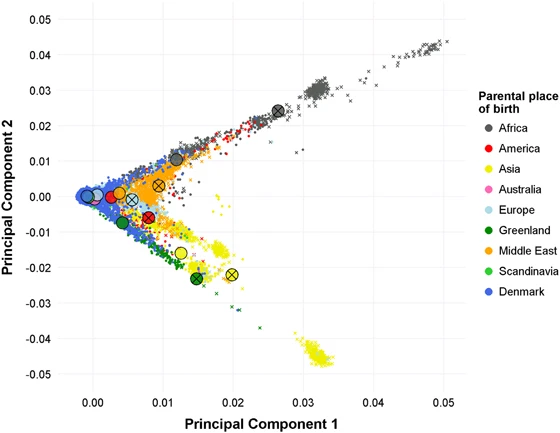
\includegraphics[width=10cm]{methods/iPSYCH_PCPlot.png}
	\caption[Scatter plot of the first two principal components of iPSYCH 
	participants coloured by parental country of birth]{The plot is provided without modification from the original paper describing 
	iPSYCH \cite{pedersen2018ipsych2012} \textbf{TODO:is it okay 
	to use a plot like this? Florian seems to think so}. The first two principal components have been 
	plotted for the iPSYCH participants and coloured according to the parent's 
	country of birth. The large circles indicate the mean values of a given 
	genetic ancestry group. The circles with a cross represent the individuals 
	where both parents are born in the region indicated by the colour, and no 
	cross means only one parent was.}
	\label{fig:ipsych_PCPlot}
\end{wrapfigure}


The above solution works well if only local subpopulations are present in an otherwise homogeneous population. A problem may arise if there are two or more genetic ancestries, as the PCs may not be able to properly account for such stratification. As a results, it seems prudent to highlight this particular cause of population stratification. Analysing different ancestries together in a GWAS is not commonly done. This is because different ancestries may have different minor allele frequencies for certain SNPs, altogether different variants on certain positions, etc.\cite{helgason2005icelandic}. Therefore, the most common way to deal with different genetic ancestries in a genotyped data set is to identify a genetically homogenous subset and perform the association analysis in the homogeneous subpopulation. There have been methods proposed that can account for genetic ancestry such as Tractor\cite{atkinson2021tractor}, but they have not been widely adopted yet. 

A homogenous subpopulation can be identified by performing a PCA on all the available individuals and calculating a robust Mahalanobis distance on the first, e.g.\ 20 PCs, and removing anyone above a certain threshold\cite{prive2020efficient}. An illustration of the feasibility of identifying the genetic ancestry for the iPSYCH participants can be seen in \cref{fig:ipsych_PCPlot}.

\subsubsection{Relatedness}
Similar to population stratification, relatedness is a common cause of spurious associations. The mechanism behind why relatedness leads to these spurious associations is a little different. If related individuals are in the same analysis, then some individuals are more alike than one would expect if they were drawn at random. Due to this, deviations from the null distribution are likely to occur, not due to the SNP's effect, but rather the sampling. For a Wald test deviation could be expressed as a downwardly biased variance estimate, which leads to inflated test statistics, as the test statistics is the effect estimate divided by the standard error \cite{astle2009population,voight2005confounding,sillanpaa2011overview}. 

There are two common ways to deal with relatedness in a GWAS setting. The first and simplest way is to identify the related individuals and removing them from the analysis. This is effective, but has the downside of reducing the sample size. The second and more involved way is to include the in-sample relatedness (sometimes also called cryptic relatedness) in the model being used for association. In a linear regression setting, the most common way to account for the cryptic relatedness is by using a linear mixed model, where a random effect that models the genotype correlation is added (see \cref{sec:GWAS:LinReg} for details). The random effect is able to account for the covariance structure of the individuals, which is how relatedness affects associations with higher than expected correlations\cite{yu2006unified, kang2008efficient}. The cryptic relatedness is accounted for by having the covariance structure of the random effect follow the GRM.

If one decides to remove the related individuals instead, then there are several ways to identify the related individuals, with the two most common ways being the GRM and identity by descent(IBD)\textbf{TODO: REF TO HOW THESE ARE DONE? LOOK AT GCTA AND PLINK PAPERS}. The GRM consists of the correlation between individual's genotypes, where a value of $ 1 $ corresponds to monozygotic twins or duplicate samples, $ 0.5 $ to a parent-offspring or sibling relationship, etc.. %If filtering is performed prior to the association test, the relatedness threshold is usually set to $ 2^{-2.5} \approx 0.177 $ when removing $ 2^{nd} $ degree relatives or closer, or $ 2^{-3.5} \approx 0.088 $ when removing $ 3^{rd} $ degree relatives, etc. Filtering for relatedness with IBD is very similar to how it is done with the GRM. 
An IBD approach for identifying relatedness is provided by the KING software\cite{manichaikul2010robust}, and a GRM based approach is provided by the GCTA software \cite{yang2011gcta}. Both ways of estimating relatedness is also implemented in the PLINK software\cite{chang2015second,purcell2007plink}


\subsubsection{Multiple testing correction}
A GWAS consists of testing each available SNP for an association with the phenotype of interest. This means several million tests are often performed. A classical statical approach to hypothesis testing means a test has a significance threshold denoted by $ \alpha $, which is most commonly $ 5\% $. If the p-value is below $ \alpha $, the null hypothesis is rejected and the alternative hypothesis is accepted. Due to the p-values being uniformly distributed under the null hypothesis, we will expect to have $ (100\times \alpha) \%$ of the tests performed rejects the null hypothesis purely by chance. There are ways to account for this. The most common multiple testing correction method used in GWAS is the Bonferroni correction\cite{balding2006tutorial,rice2008methods}. As a motivation for the Bonferroni correction, let $ n $ independent tests be given, then the family-wide error rate $ \bar{\alpha} $, meaning the probability of seeing at least one false positive across all $ n $ tests, is given by

\begin{equation} \label{eq:bonferroni}
\bar{\alpha} = 1 - (1-\alpha)^n 
\end{equation}
$ \alpha$ is the per-test significance level. This leads to the Bonferroni correction $ \alpha_{bf} =  \alpha/n $. By comparing the repeated tests against $ \alpha_{bf} $ instead of $ \alpha $, the expected number of false positives will remain $ \alpha $ across all tests performed, thereby controlling the number of type-1 errors. In a GWAS setting, it is common to assume 1 million independent tests are performed\cite{pe2008estimation}, which leads to a genome-wide significance threshold of $ 5 \times 10^{-8} $.



\subsubsection{Unbalanced case-control phenotypes}
If a case-control phenotype is used in a GWAS, where the case-control ratio exceeds $ 1{:}80 $, it may have significantly inflated test statistics\cite{zhou2018efficiently,}. Ma et al. frames the same problem in terms of minor allele count(MAC) and suggests a MAC of $ 400 $ or higher for a well-balanced test\cite{ma2013recommended}. The unbalanced case-control phenotypes lead to inflated test statistics because the tests often rely on asymptotic distribution assumptions. These assumptions do not seem to hold if the MAC is low or if the case-control ratio is unbalanced. While BOLT-LMM provided an efficient implementation for linear mixed models, further study of the software have revealed that it suffers from inflated test statistics.

Methods such as SAIGE\cite{zhou2018efficiently}, SPACox\cite{bi2020fast}, GATE\cite{dey2022efficient}, and REGENEIE\cite{mbatchou2021computationally} have been proposed to combat the inflation of test statistics due to deviations from the asymptotic distribution assumptions. A strategy most of these methods utilise is the saddle point approximation (SPA)\cite{daniels1954saddlepoint,kuonen1999miscellanea}. One of the advantages of using SPA is that it provides good control of Type 1 error, even for unbalanced case-control phenotypes and as such do not suffer from inflation of the test statistic in such cases\cite{mbatchou2021computationally}.

SPA can efficiently estimate CDF probabilities from only the cumulant generating function, $ K $. Let $ T $ be the test statistics of a commonly used GWAS association test statistics, then the CDF of $ T $, which is needed to calculate p-values, is approximated by

\begin{equation}
P(T < x) = \Phi\left( w + w^{-1} \log(v/w)\right)
\end{equation}
with $ \Phi $ denotes the standard normal CDF and
\begin{equation}
w = \text{sign}(\hat{\zeta})\left[2\left(\hat{\zeta} x - K(\hat{\zeta})\right) \right]^{1/2},
 \qquad 
v = \hat{\zeta}\sqrt{K^{''}(\hat{\zeta})}
\end{equation}
where $ \hat{\zeta} = \hat{\zeta}(x) $ is the solution to $ K^{'}(\hat{\zeta}) = x $, with $ K^{'} $ and $ K^{''} $ denoting the first and second derivative of the cumulant generating function. If the test statistic is close to the mean, a normal approximation is usually good. As a result, the normal distribution is often used if the test statistic is within two standard deviations of the mean, and the SPA otherwise.



\subsection{Computational efficiency} \label{sec:computationalEfficiency}
This section will cover some of the common computational or mathematical tricks used to speed up GWAS. Biobanks have been steadily increasing in size. it is therefore more important than ever to have as efficient methods as possible, since we would otherwise risk having data sets too large to properly analyse. We will briefly describe how one can avoid estimating the effect sizes of covariates that have been included in the model and tricks on how to avoid inverting matrices. 



\subsubsection{Projecting covariates}
There is a computational cost involved in estimating the effects of the covariates. Therefore, the most efficient way to account for the covariates without directly calculating their effect in each regression is to project them out of the predictor and the response of interest in \cref{eq:baseGWAS} \cite{sikorska2013gwas}. For the sake of completeness, we will present how to regress out the covariates as they were presented by Sikorska et al.\cite{sikorska2013gwas}. 

Considering the residual sum of squares(RSS) for \cref{eq:baseGWAS}, we get 

\begin{align}
	RSS =& \left( y - \beta G_j - X\gamma \right)^T\left( y - \beta G_j - X\gamma \right) \\
	=& y^T y - 2\beta y^T G_j - 2y^TX\gamma - \beta^2 G_j^TG_j + 2\beta G_j^T X + \gamma^T X^T X \gamma.
\end{align}
Recall that $ X\gamma $ is a vector of dimension $ N \times 1 $, which means $ y^T X \gamma $ is an inner product and inner products are symmetric. Differentiating the residual sum of squares with respect to $ \beta $ and $ \gamma $ yields

\begin{align}
	\dfrac{\partial}{\partial \beta} (RSS) = -2y^TG + 2\beta G_j^TG_j + 2G_j^T X\gamma \\
	\dfrac{\partial}{\partial \gamma} (RSS)  = -2y^TX + 2\beta G^T_j X + 2X^TX\gamma 
\end{align}
Setting these expressions equal to $ 0 $, we get
\begin{align}
	G_j^T G_j \beta +  G_j^T X \gamma =  G_j^T y  \label{eq:covregress1}\\ 
	X^T G_j \beta + X^T X \gamma =  X^Ty \label{eq:covregress2}
\end{align}
This means the matrix notation of the least squares solution to \cref{eq:baseGWAS} is given by 
\begin{equation}
	\begin{pmatrix}
		G_j^T G_j & G_j^T X \\
		X^T G_j & X^T X
	\end{pmatrix}
	\begin{pmatrix}
		\hat{\beta} \\
		\hat{\gamma}
	\end{pmatrix} = 
	\begin{pmatrix}
		G_j^T y \\
		X^T y
	\end{pmatrix}.
\end{equation}
and we will let $ \hat{\beta} $ and $ \hat{\gamma} $ denote solutions to the least squares equations. However, we are interested in an expression that does not depend on the covariates. From here we isolate $ \hat{\gamma} $ in \cref{eq:covregress2} and get $ \hat{\gamma} = (X^TX)^{-1}(X^Ty - \hat{\beta} X^TG_j) $, which is then inserted in to \cref{eq:covregress1} 

\begin{equation}
	G^T_j y = G_j^TG_j + G_j^TX (X^TX)^{-1}(X^Ty - \hat{\beta} X^TG_j).
\end{equation}
By isolating terms related to $ y $ on the left hand side and term related to $ \hat{\beta} $ on the right hand side we get the following

\begin{equation} \label{eq:GWASprojection}
	G_j^T(y - X(X^TX)^{-1}X^Ty) = G_j^T(G_j - X(X^TX)^{-1}X^TG_j) \hat{\beta}.
\end{equation}
Recall that $ X(X^TX)^{-1}X^T $ denotes the projection onto the space spanned by the matrix $ X $. From here, we will introduce transformations given by 
\begin{align}
	y^\ast = y - X(X^TX)^{-1}X^Ty & & & G_j^{\ast} = G_j - X(X^TX)^{-1}X^TG_j.
\end{align}
The transformations remove the effect of the covariates in $ X $ from the response and predictor of interest. Using the properties of projections, \cref{eq:GWASprojection}, and the transformations, we find that 

\begin{equation}
	\left( G_j^{\ast} \right)^T G_j^{\ast} \hat{\beta} = G_j^T G_j^{\ast} \hat{\beta} \stackrel{\ref{eq:GWASprojection}}{=} G_j^T y^{\ast} = \left( G_j^{\ast} \right)^T y^{\ast}.
\end{equation}
The normal equation for systems of equations of the form $ Ax=b $ say that $ \hat{\beta} $ is a solution to a new univariate regression given by

\begin{align}\label{eq:univarGWAS}
	y^\ast = \hat{\beta} G_j^{\ast} + \varepsilon&   &\text{with simplified solution}&  &\hat{\beta} = \dfrac{\left( G_j^{\ast} \right)^T y^{\ast}}{\left( G_j^{\ast} \right)^T G_j^{\ast}}.
\end{align}
With the projection, the effect of the covariates have been removed from the outcome and the predictor, i.e. the phenotype and the 
genotype do \textit{not} depend on $ \gamma $ any more. Therefore, the calculations have been simplified and the calculations for the 
projection matrix only has to be performed once. Accounting for the covariate's effect in the phenotype also only has to be done once, 
the removal of the covariate's effect on the SNP has to be done for each SNP separately.

One of the most common ways to perform the test is with a Wald test $ Z = \hat{\beta}/\text{se}(\hat{\beta}) \sim N(0,1)$. 
\textbf{TODO: what is se(beta)}
\textbf{TODO: Florian's thesis deals with speeding up computations even further, mention this too?}


\subsubsection{Avoiding large matrix inversions}

In this section, we will focus on ways of improving the computational efficiency of linear mixed models. First, a short introduction to which calculations are the most computationally intensive will be provided. Secondly, a way to circumvent the direct calculations will be provided. We will use the mixed model implementation in BOLT-LMM as an example.

BOLT-LMM utilises a stochastic restricted maximum likelihood (REML) approach to estimate the variance components from \cref{eq:baseMixedModelGWAS}. The approach is called stochastic, since it utilises Monte Carlo sampling. The estimate acquired is a REML estimate, as all covariates have already been projected out of the phenotype vector, $ y $, the genotypes, $ G_j $, and the environment, $ \varepsilon $. This means degrees of freedom been reduced by $ C $, which is the rank of the design matrix $ X $. On top of this, all observations will now belong to an $ N-C $ dimensional subspace of $ \mathbb{R}^{N} $, and the distribution of the environmental term is now changed to $ \varepsilon \sim N(\mathbf{0}, \sigma_e^2 P)$, where $ P $ denotes the projection matrix on the space spanned by $ X $. Recall that a projection is symmetric and idempotent, hence only $ P $ is left in the covariance matrix of $ \varepsilon $. 

In this reduced setup, we will present how the variance components are estimated in an efficient manner under the infinitesimal model. First, we will reframe the problem in terms of a Bayesian setting where all of the covariates have been projected out. In the notation of \cref{eq:baseMixedModelGWAS}, we have

\begin{equation}\label{eq:bolt:infinitesimalModel}
y = Z\beta + \varepsilon, \qquad cov(y) = \sigma_g^2 K + \sigma_e^2 P
\end{equation}
where each SNP's effect has the prior $ \beta_j \sim N(0, \sigma_j^2)$ with $\sigma_j^2 = \sigma_g^2 / M $. The \textit{stochastic} REML then simulates observations under the model in \cref{eq:bolt:infinitesimalModel} and attempts to find a solution to an equivalent problem. With a slight abuse of notation of $ \lVert \varepsilon \rVert^2$ and  $ \lVert \beta \rVert^2$, we can phrase the alternative problem that we will solve as

\begin{equation} \label{eq:bolt:AlternativeMMEProblem}
E\left[ \sum \hat{\varepsilon}^2_{rand} \right] = \sum \hat{\varepsilon}^2_{data}, \qquad E\left[ \sum \hat{\beta}^2_{rand} \right] = 
\sum \hat{\beta}^2_{data}.
\end{equation}
Here $ \hat{\beta}^2_{data} $ and $ \hat{\varepsilon}^2_{data} $ are the BLUP estimates in \cref{eq:bolt:infinitesimalModel}. The 
terms in the expectation are $ \hat{\beta}^2_{rand} $ and $ \hat{\varepsilon}^2_{rand} $ and they are simulated values under the same model, but with a known and fixed $ \sigma_g^2 $ and $ \sigma_e^2 $. The simulated values are given by

\begin{equation} \label{eq:bolt:AlternativeMMEobs}
y_{rand} = Z \beta_{rand} + \varepsilon_{rand}, \qquad \beta_{rand,j} \sim N(0, \sigma_j^2),  \qquad \varepsilon_{rand,j} \sim N(0, 
\sigma_e^2).
\end{equation} 
Hence, the left hand side of \cref{eq:bolt:AlternativeMMEProblem} can be estimated by samples generated from 
\cref{eq:bolt:AlternativeMMEobs} with fixed and known variance components and the right hand side can be estimated with a BLUP estimator. This setup allows for iteratively calculating the BLUP estimates and estimating the variance components. We will outline how this iterative scheme is performed now. First, we will assume that we have $ \sigma_g^2 $ and $ \sigma_e^2 $ known and fixed. Then, we will define the following 

\begin{align}
	\delta := \dfrac{\sigma_e^2}{\sigma_g^2}, \qquad H := K + \delta I_N.
\end{align}
From here, the BLUP estimates are given by
\begin{align} \label{eq:bolt:iterativeBLUP}
	\hat{\beta} = \dfrac{1}{M}Z^T H^{-1} y,  \qquad  \hat{e} = \delta H^{-1}y
\end{align}
Note that the BLUP estimates are constant for a fixed $ \delta $. With this, we can calculate the BLUP estimates. Next, we need a way to find estimates of the variance components, $ \sigma_g^2 $ and $ \sigma_e^2 $. We will rephrase \cref{eq:bolt:AlternativeMMEProblem} as a single equation that depends on $ \delta $ with 

\begin{equation}
\dfrac
{E\left[ \sum \hat{\beta}^2_{rand} \right]}
{E\left[ \sum \hat{\varepsilon}^2_{rand} \right]}
 =
\dfrac
{\sum \hat{\beta}^2_{data}}
{\sum \hat{\varepsilon}^2_{data}}.
\end{equation}
where we can scale $ \sigma_g^2 $ such that it matches the observed data. From here, we can get $ 1 $ on the left hand side of the rephrase equation above, and take the logarithm on both sides to get

\begin{equation}\label{eq:bolt:iterativeRatio}
f_{reml}(\log(\delta)) 
:= \log 
\left(
\dfrac
{
E\left[ \sum \hat{\varepsilon}^2_{rand} \right]	
\sum \hat{\beta}^2_{data}
}
{
\sum \hat{\varepsilon}^2_{data}
E\left[ \sum \hat{\beta}^2_{rand} \right]
}
\right).
\end{equation}
As a result, we have to find a value of $ \delta $ which satisfy $ f_{reml}(\log(\delta)) = 0$. We will not elaborate on the details of how this is done, but it involves using the secant method and a sampling strategy similar to the one used above for the BLUP estimate. In summary, estimating the variance components in a mixed model, as presented in BOLT-LMM, means calculating the BLUP estimates in \cref{eq:bolt:iterativeBLUP} and finding $ \delta $ that solves \cref{eq:bolt:iterativeRatio}. However, the calculations needed to perform the iterative scheme require inverting a matrix. Matrix inversion is computationally expensive and has computational complexity of $ O(N^3) $ if calculated naively. Other strategies have been suggested, which allows for a computational complexity of $ O(NM^2) $ or $ O(N^2M) $ \cite{svishcheva2012rapid,lippert2011fast}. The strategy employed in BOLT-LMM has a computational complexity of $ O(NM) $, which makes it much faster. 

The variance of the phenotype, as seen in \cref{eq:MixedModelGWASCovariance} or in the iterative scheme as \cref{eq:bolt:iterativeBLUP} will have to be inverted, if calculated naively. We can efficiently perform calculations of the form $ H^{-1}y $ and circumvent the inversion by not directly forming $ H $, but instead considering its terms, $ ZZ^T / M$ and $ \delta I_N$. If we multiply with some vector, $ q $, from the right, then it is only the GRM term that is computationally expensive. However, we can express it in the following way

\begin{equation}
ZZ^T q = \sum_i \left( Z_i Z_i^T\right) q = \sum_i  Z_i \left(Z_i^T q\right) 
\end{equation}
The first equation expresses $ Z Z^T $ as the sum of the outer products of columns of $ Z $ and the second as a sum of vectors times a scalar, where the scalar is the result of an inner product between the $ i^{th} $ column of $ Z $ and the given vector $ q $. This reformation of the product $ Z Z^T q$ has computational complexity $ O(NM) $.

\textbf{TODO: THEY ACTUALLY JUST SOLVE Vx = b, WHICH IS THE SAME AS DIRECTLY CALCULATING x = INV(V)b}

\textbf{TODO: i am not sure, but it almost seem like it is suggested that $ (A + B)^{-1} = A^{-1} + B^{-1} $, which i do not think holds generally. they specifically say in the suppNotes that they do not form H and only consider the terms individually and multiply from the right with a vector.}


%BOLT-LMM utilise a mixed linear model with a Gaussian mixture prior, which allows for a non-infinitesimal model. 
%BOLT steps
%(1a) estimation of variance parameters; 
%circumvents spectral decomposition with stochastic approximation algorithm instead. it requires finding a solution to a linear systems of mixed-model equations instead, which is done by conjugate gradient iteration.
%(1b) computation of infinitesimal mixed-model association statistics (BOLT-LMM-inf); 
%circumvents spectral decomposition by introducing a new retrospective mixed-model association statistic similar to GRAMMAR-Gamma10 and MASTOR23, which we compute—up to a calibration constant—using only the solutions to linear systems of equations. We estimate the calibration constant by computing the new statistic and comparing it to the standard prospective mixed-model statistic at a random subset of SNPs; this step can likewise be accomplished efficiently using conjugate gradient iteration. This procedure is similar in spirit to GRAMMAR-Gamma calibration but requires only O(MN) time iterations.
%(2a) estimation of Gaussian mixture-model parameters; 
%
%(2b) computation of Gaussian mixture-model association statistics (BOLT-LMM)

\subsection{Increasing power in GWAS}

Increasing power to detect the true associations has been another primary focus of GWAS method developments. The leap from linear regression to a linear mixed model is expected to provide a power increase \cite{loh2015efficient}. The increase comes from modelling the covariance structure present in the data, which is not possible for linear regression. As the covariance structure is modelled, it is no longer necessary to remove individuals due to relatedness or population stratification. This has the additional benefit that the sample size increase, which in turn increases power. 

Another source of power improvement is accounting for the effect of other SNPs. When one accounts for other SNPs in this manner, it essentially means a reduction in the residual variance of the phenotype, which is also why it has been referred to as \textit{denoising} the phenotype\cite{aschard2015adjusting}. Reducing the residual variance of the phenotype has proven to be an effect way to increase power in a GWAS, and we will briefly present how it can be done. Again, we will use BOLT-LMM as an example.

In BOLT-LMM, they utilise an infinitesimal model and a Bayesian model with mixture Gaussian priors. The mixture model allows for a non-infinitesimal model to be used, as some SNPs will be set to $ 0 $ and the variance for groups of SNPs can vary.  In a linear mixed model setup, as seen in \cref{sec:GWAS:LinReg} and with the covariance of $ y $ given as $V = \sigma_g^2G^TG/M + \sigma_e^2I_N $, the test statistic is given by

\begin{equation}\label{eq:boltLMMchisq}
\chi^2_{LMM} = \dfrac{(G_j^TV^{-1}y)^2}{G_j^TV^{-1}G_j}
\end{equation}
with $ \sigma_g^2 $ and $ \sigma_e^2 $ estimates under the null hypothesis $ H_0{\,:\,} \beta = 0 $. However, performing a test in this way means accounting for the same SNPs more than once, as the SNP of interest will also be present in the GRM. We can avoid it by removing the chromosome that the $ j^{th} $ SNP belongs to from the GRM calculations. This is called leave-one-chromosome-out (LOCO). We will denote the LOCO GRM as $ V_{LOCO} = (G_{LOCO})^TG_{LOCO}/M_{LOCO}$, where $ G_{LOCO} $ is the SNP that remain after removing the $ j^{th} $ SNP's chromosome and $ M_{LOCO} $ is the number of SNPs after removing the same chromosome. We get the LOCO test statistic to be

\begin{equation}\label{eq:boltLMMchisqLOCO}
\chi^2_{LOCO} = \dfrac{(G_j^TV_{LOCO}^{-1}y)^2}{G_j^TV_{LOCO}^{-1}G_j}
\end{equation}
Notably, this means calculating a $ V_{LOCO} $ for each chromosome. The BOLT-LMM infinitesimal model has a test statistic that is given by

\begin{align}\label{eq:boltLMMinfchisq}
\chi^2_{BOLT-INF} = \dfrac{(G_j^TV_{LOCO}^{-1}y)^2}{c_{inf}} & &c_{inf} = \dfrac{\text{mean}((G_j^TV_{LOCO}^{-1}y)^2)}{\text{mean}(\chi^2_{LOCO})}
\end{align}
Where $ c_{inf} $ is chosen such that $ \text{mean}(\chi^2_{BOLT-INF}) = \text{mean}(\chi^2_{LOCO})$. The constant $ c_{inf} $ is estimated from $ 30 $ pseudorandom SNPs. As we are able to account for some of the other SNPs with the LOCO testing scheme in BOLT-LMM, we achieve a power increase.

When introducing the Gaussian mixture prior, they generalise the test statistic as

\begin{equation}\label{eq:boltMixturePriorTestChisq}
\chi^2_{BOLT-LMM} = \dfrac{\left( G_j^T y_{residual}\right)^2}{c}
\end{equation}
where $ y_{residual} $ is a residual phenotype vector obtained after fitting a Gaussian mixture extension of the standard LMM. The model used to fit the phenotype is still using LOCO, but to ease notation, the notation has been suppressed. The calibration factor $ c $ is chosen such that the intercept of $ \chi^2_{BOLT-LMM} $ with LD score regression\cite{bulik2015ld} model matches the intercept of the properly calibrated $ \chi^2_{BOLT-INF} $.

The test statistic for the non-infinitesimal model require calculating the residualised phenotype $ y_{residual} $. Next we will describe how those are obtained. Under a Bayesian framework, the null model associated with \cref{eq:boltLMMchisqLOCO} is given as

\begin{equation}\label{eq:boltBayesLMMWithPrior}
y = G_{LOCO} \beta_{LOCO} + \varepsilon \qquad \beta_j \sim N(0, \sigma^2_g /M_{LOCO}), \qquad \varepsilon \sim N(\mathbf{0},\sigma_e^2I_N)
\end{equation}
Note that the model is infinitesimal as all SNPs $ \beta_j $ follow the same distribution. The generalisation to a Gaussian mixture prior means replacing the prior for $ \beta_j $ with 

\begin{equation}
\beta_j \sim
\begin{cases}
N(0, \sigma^2_{g1}) & \text{with probability } p \\
N(0, \sigma^2_{g2}) & \text{with probability } 1-p
\end{cases}
\end{equation}
This prior is sometimes called a spike-and-slab prior, since one of the variances $ \sigma^2_{g1} $ or $  \sigma^2_{g2} $ may be very large while the other may be very small. This results in two normal distributions, one very concentrated around $ 0 $, and another that allows for large variations in effect sizes. If illustrated, this looks like a spike around $ 0 $, and a slab covering a large area, hence the name.

The effect sizes, $ \beta_j $, are estimated from \cref{eq:boltBayesLMMWithPrior}, and the residualised phenotype under the Gaussian mixture prior vector is calculated as

\begin{equation}
y_{residual} = y - G_{LOCO}\beta_{LOCO}
\end{equation}
The residualised phenotype vector, $ y_{residual} $, is then used in \cref{eq:boltMixturePriorTestChisq}. In summary, using the infinitesimal model with the LOCO scheme, increases power compared to simple linear regression. Using the mixture prior, increases the effective sample size by an additional $ 25\% $ compared to the infinitesimal model.



\subsection{Notable methodological advancements}
This section provides a non-exhaustive list of methodological advances proposed for GWAS. The list aims to highlight key advances that have been made by either providing computational feasibility for a certain type of analysis, use of a more complex model, or both. Notable GWAS methods are presented in \cref{table:GWASoverview}. 

\begin{table}[h]
	\centering
	\begin{tabularx}{\textwidth}{l X l}
		\hline
		Software	&	Notable advancement		&	Model \\
		\hline
		PLINK\cite{chang2015second,purcell2007plink}	&
		Highly scalable linear and logistic regression \& Data management and standardized a binary storage format	&
		Linear \& logistic regression	\\
		BOLT\cite{loh2015efficient}	&
		Efficient linear mixed model for UKBB sized data that accounts for cryptic relatedness \& increases power	&
		Linear mixed model	\\
		SPACox\cite{bi2020fast}	&	
		Saddle point approximation based proportional hazards model for UKBB sized data &
		Cox proportional hazards \\
		GATE\cite{dey2022efficient}	&
		Saddle point approximation based frailty model for UKBB sized data	&
		Frailty model \\
		\hline
	\end{tabularx}
	\caption{Overview of notable GWAS methods}
	\label{table:GWASoverview}
\end{table}

